\begin{figure}[h] 
\centering 
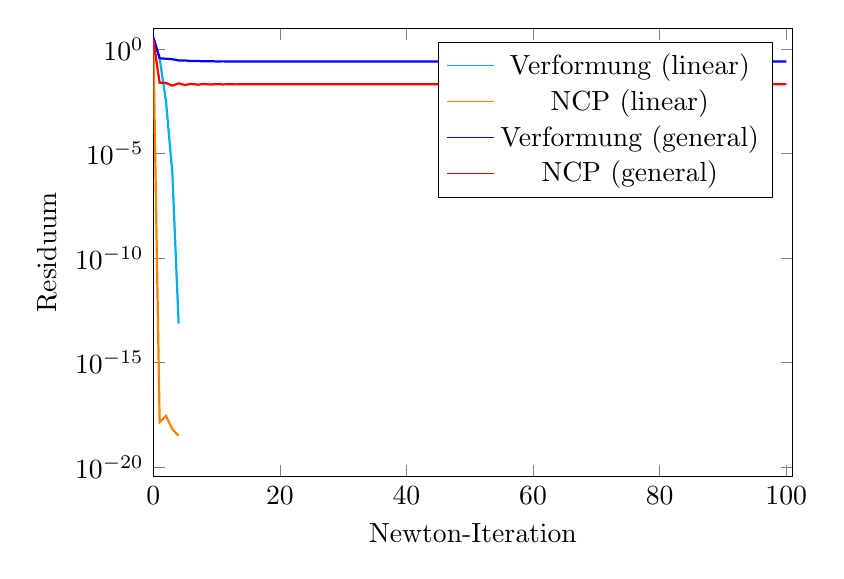
\begin{tikzpicture}[every plot/.append style={thick}] 
\begin{axis}[ 
label style={font=\normalsize}, 
xlabel={Newton-Iteration}, 
ylabel={Residuum}, 
xmin=0, xmax=101, 
ymode=log, 
ymin=0, ymax=10, 
width=0.8\textwidth, 
height=0.6\textwidth, 
legend pos=north east, 
legend style={cells={align=left}}, 
grid style=dashed, 
] 
\addplot[ 
color=cyan, 
] 
coordinates { 
(0, 3.61e+00)(1, 3.64e-01)(2, 3.23e-03)(3, 1.26e-06)(4, 7.23e-14)}; 
\addlegendentry{Verformung (linear)} 
\addplot[ 
color=orange, 
] 
coordinates { 
(0, 2.75e+00)(1, 1.39e-18)(2, 2.73e-18)(3, 6.51e-19)(4, 3.07e-19)}; 
\addlegendentry{NCP (linear)} 
\addplot[ 
color=blue, 
] 
coordinates { 
(0, 3.61e+00)(1, 3.64e-01)(2, 3.46e-01)(3, 3.28e-01)(4, 2.88e-01)(5, 2.88e-01)(6, 2.67e-01)(7, 2.70e-01)(8, 2.59e-01)(9, 2.63e-01)(10, 2.57e-01)(11, 2.59e-01)(12, 2.55e-01)(13, 2.58e-01)(14, 2.55e-01)(15, 2.57e-01)(16, 2.55e-01)(17, 2.56e-01)(18, 2.55e-01)(19, 2.56e-01)(20, 2.55e-01)(21, 2.56e-01)(22, 2.55e-01)(23, 2.56e-01)(24, 2.55e-01)(25, 2.56e-01)(26, 2.55e-01)(27, 2.56e-01)(28, 2.55e-01)(29, 2.56e-01)(30, 2.55e-01)(31, 2.56e-01)(32, 2.55e-01)(33, 2.56e-01)(34, 2.55e-01)(35, 2.56e-01)(36, 2.55e-01)(37, 2.56e-01)(38, 2.55e-01)(39, 2.56e-01)(40, 2.55e-01)(41, 2.56e-01)(42, 2.55e-01)(43, 2.56e-01)(44, 2.55e-01)(45, 2.56e-01)(46, 2.55e-01)(47, 2.56e-01)(48, 2.55e-01)(49, 2.56e-01)(50, 2.55e-01)(51, 2.56e-01)(52, 2.55e-01)(53, 2.56e-01)(54, 2.55e-01)(55, 2.56e-01)(56, 2.55e-01)(57, 2.56e-01)(58, 2.55e-01)(59, 2.56e-01)(60, 2.55e-01)(61, 2.56e-01)(62, 2.55e-01)(63, 2.56e-01)(64, 2.55e-01)(65, 2.56e-01)(66, 2.55e-01)(67, 2.56e-01)(68, 2.55e-01)(69, 2.56e-01)(70, 2.55e-01)(71, 2.56e-01)(72, 2.55e-01)(73, 2.56e-01)(74, 2.55e-01)(75, 2.56e-01)(76, 2.55e-01)(77, 2.56e-01)(78, 2.55e-01)(79, 2.56e-01)(80, 2.55e-01)(81, 2.56e-01)(82, 2.55e-01)(83, 2.56e-01)(84, 2.55e-01)(85, 2.56e-01)(86, 2.55e-01)(87, 2.56e-01)(88, 2.55e-01)(89, 2.56e-01)(90, 2.55e-01)(91, 2.56e-01)(92, 2.55e-01)(93, 2.56e-01)(94, 2.55e-01)(95, 2.56e-01)(96, 2.55e-01)(97, 2.56e-01)(98, 2.55e-01)(99, 2.56e-01)(100, 2.55e-01)}; 
\addlegendentry{Verformung (general)} 
\addplot[ 
color=red, 
] 
coordinates { 
(0, 2.75e+00)(1, 2.46e-02)(2, 2.39e-02)(3, 1.79e-02)(4, 2.28e-02)(5, 1.91e-02)(6, 2.19e-02)(7, 1.98e-02)(8, 2.14e-02)(9, 2.02e-02)(10, 2.11e-02)(11, 2.04e-02)(12, 2.09e-02)(13, 2.05e-02)(14, 2.08e-02)(15, 2.06e-02)(16, 2.08e-02)(17, 2.06e-02)(18, 2.07e-02)(19, 2.07e-02)(20, 2.07e-02)(21, 2.07e-02)(22, 2.07e-02)(23, 2.07e-02)(24, 2.07e-02)(25, 2.07e-02)(26, 2.07e-02)(27, 2.07e-02)(28, 2.07e-02)(29, 2.07e-02)(30, 2.07e-02)(31, 2.07e-02)(32, 2.07e-02)(33, 2.07e-02)(34, 2.07e-02)(35, 2.07e-02)(36, 2.07e-02)(37, 2.07e-02)(38, 2.07e-02)(39, 2.07e-02)(40, 2.07e-02)(41, 2.07e-02)(42, 2.07e-02)(43, 2.07e-02)(44, 2.07e-02)(45, 2.07e-02)(46, 2.07e-02)(47, 2.07e-02)(48, 2.07e-02)(49, 2.07e-02)(50, 2.07e-02)(51, 2.07e-02)(52, 2.07e-02)(53, 2.07e-02)(54, 2.07e-02)(55, 2.07e-02)(56, 2.07e-02)(57, 2.07e-02)(58, 2.07e-02)(59, 2.07e-02)(60, 2.07e-02)(61, 2.07e-02)(62, 2.07e-02)(63, 2.07e-02)(64, 2.07e-02)(65, 2.07e-02)(66, 2.07e-02)(67, 2.07e-02)(68, 2.07e-02)(69, 2.07e-02)(70, 2.07e-02)(71, 2.07e-02)(72, 2.07e-02)(73, 2.07e-02)(74, 2.07e-02)(75, 2.07e-02)(76, 2.07e-02)(77, 2.07e-02)(78, 2.07e-02)(79, 2.07e-02)(80, 2.07e-02)(81, 2.07e-02)(82, 2.07e-02)(83, 2.07e-02)(84, 2.07e-02)(85, 2.07e-02)(86, 2.07e-02)(87, 2.07e-02)(88, 2.07e-02)(89, 2.07e-02)(90, 2.07e-02)(91, 2.07e-02)(92, 2.07e-02)(93, 2.07e-02)(94, 2.07e-02)(95, 2.07e-02)(96, 2.07e-02)(97, 2.07e-02)(98, 2.07e-02)(99, 2.07e-02)(100, 2.07e-02)}; 
\addlegendentry{NCP (general)} 
\end{axis} 
\end{tikzpicture} 
\caption{Residuen des Stoffgesetzes 'Neo Hooke' mit Hinderniss 'Hut' und 162 Freiheitsgraden für die Verschiebung.} 
\label{fiq:NeoHooke_Hut_level2} 
\end{figure} 
